\documentclass{article}
\usepackage{graphicx}
\usepackage{amssymb}
\usepackage{amsmath}
\usepackage{float}

\usepackage[margin=1in]{geometry}


\begin{document}



\title{16-720 Computer Vision: Homework 3}
\author{Xiang Zhi Tan}

\maketitle
\subsection*{Q1.1}
With the original equation, we do a first-order Taylor expension on it.
\begin{equation*}
\sum_{(x,y)\in R_{t}}(I_{t+1}(x+u,y+u) + \bigtriangledown I_{t+1}(u,v) - I_t(x,y))^2
\end{equation*}
As we are trying to minimize this equation in terms of $u$ and $v$. We then take the partial derivative in terms of $(u,v)$. That gives us
\begin{equation*}
2 \sum_{(x,y)\in R_{t}}[(\bigtriangledown I_{t+1})^T  (I_{t+1}(x+u,y+u) + \bigtriangledown I_{t+1}(u,v) - I_t(x,y))]
\end{equation*}
We ignore the leading 2 since we are minimizing the function by rearranging the function and setting it equal to 0, we will get
\begin{equation*}
0 = \sum_{(x,y)\in R_{t}}(\bigtriangledown I_{t+1})^T \times I_{t+1}(x+u,y+u) + \sum_{(x,y)\in R_{t}}(\bigtriangledown I_{t+1})^T \times \bigtriangledown I_{t+1}(u,v) - \sum_{(x,y)\in R_{t}}(\bigtriangledown I_{t+1})^T \times I_t(x,y))
\end{equation*}
Let $\Delta P = (u,v)^T$ and move everything else to the other side
\begin{equation*}
\sum_{(x,y)\in R_{t}}(\bigtriangledown I_{t+1})^T \times \bigtriangledown I_{t+1}\Delta p = \sum_{(x,y)\in R_{t}}(\bigtriangledown I_{t+1})^T \times I_t(x,y)) - \sum_{(x,y)\in R_{t}}(\bigtriangledown I_{t+1})^T \times I_{t+1}(x+u,y+u).
\end{equation*}
Now we have the form $A\Delta P = b$. $A^T A = \sum_{(x,y)\in R_{t}}(\bigtriangledown I_{t+1})^T \times \bigtriangledown I_{t+1}$. $A^T A$ is called the \textbf{Hessian} in the Lucas Kanade algorithm and individually, $A$ is called \textbf{steepest descent}.\\
For the algorithm to work. $A^TA$ has to be invertible. This is because to calculate $\Delta p$, the Hessian has to be inverted and move to the other side of the equation. Following is the derivation of the Lucas Kanade algorithm after moving the Hessian
\begin{equation*}
\Delta p = H^{-1}[\sum_{(x,y)\in R_{t}}(\bigtriangledown I_{t+1})^T \times I_t(x,y)) - \sum_{(x,y)\in R_{t}}(\bigtriangledown I_{t+1})^T \times I_{t+1}(x+u,y+u)].
\end{equation*}

\subsection*{Q1.3}
Following is the result of my Lucas-Kanade tracker at different frame locations
\begin{figure}[H]
    \centering
    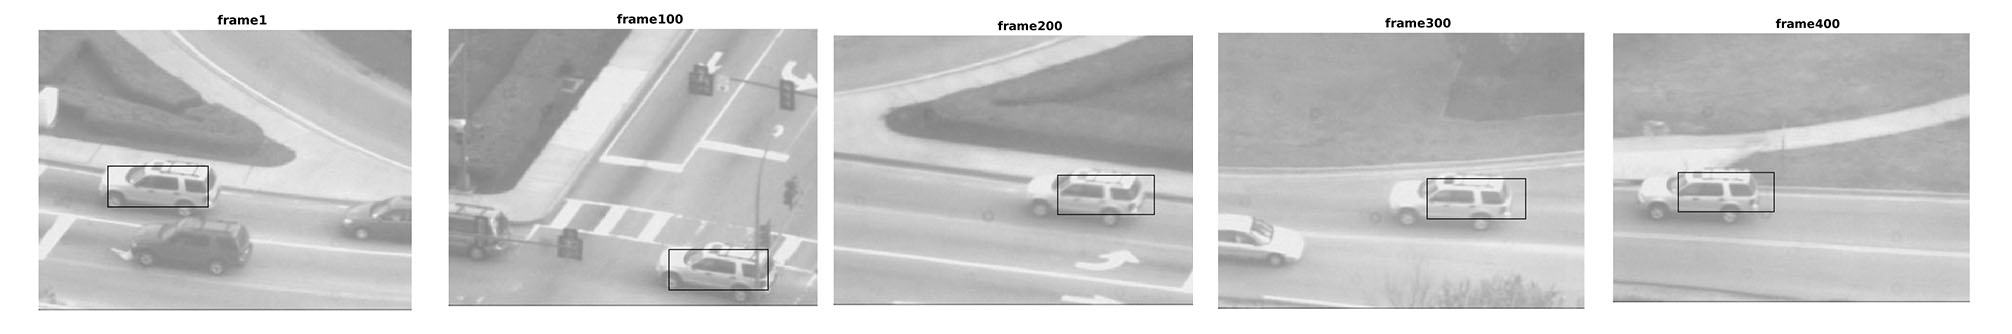
\includegraphics[width=6.5in]{./figures/fig-1-3-combined}
    \caption{The result of the tracking algorithm at frames 1,100,200,300,400}
\end{figure}
\subsection*{Q2.1}
Firstly, we can express $\sum^{k}_{c=1}w_cB_c$ in terms of a matrix.
\begin{equation*}
\begin{pmatrix}
w_1 & w_2 & ... & w_k
\end{pmatrix}
\begin{pmatrix}
|&|&..&|\\
B_1&B_2&..&B_k\\
|&|&..&|\\
\end{pmatrix}
\end{equation*}
Let's set them as $WB$. Now we rearrange the equation because $B$ is invertible due to it's orthogonal properties.
\begin{equation*}
W = B^{-1}(I_{t+1} - I_{t})
\end{equation*}
\subsection*{Q2.2}
Both my \textbf{LucasKanadeBasis} and \textbf{LucasKanade} have nearly identical performance on both the original and extended dataset. I was unable to distinguish which algorithm perform worse(they both were able to track the object around correctly with slight drift in the end) I included the recorded rects in the file \textbf{sylvseqrects.mat} and \textbf{sylvseqextrects.mat}\\
Below are the images showing the result of the two algorithms. You can see that there was only a small difference at frame 1200 and 1100 where there is some slight green outline showing the original lucas kanade's rectangle.
\begin{figure}[H]
    \centering
    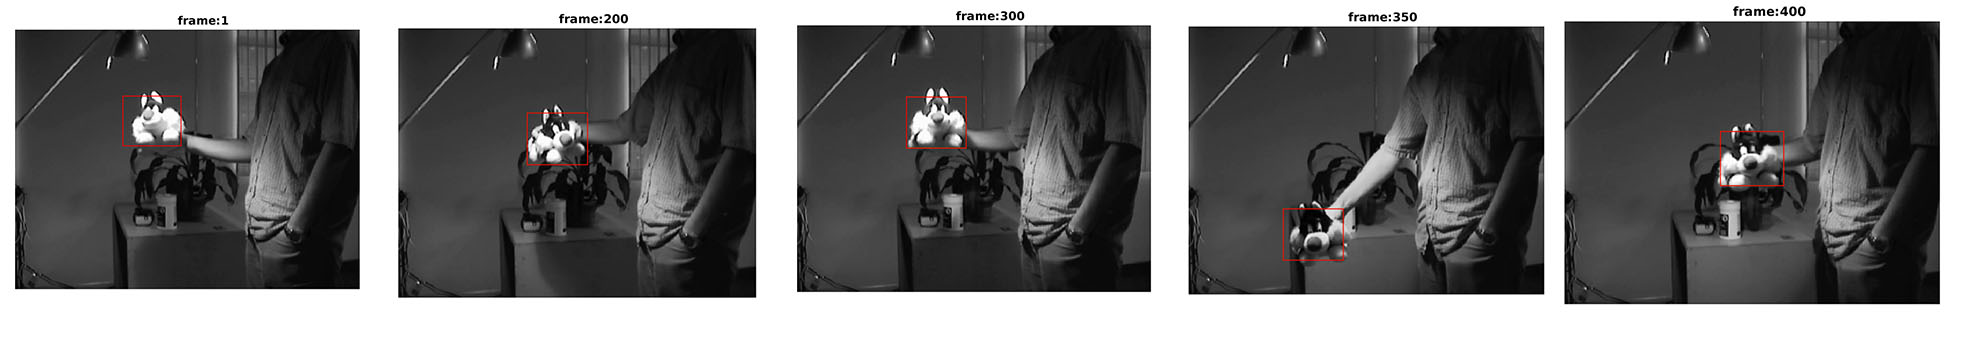
\includegraphics[width=6.5in]{./figures/p2}
    \caption{The result of the LucasKanadeBasis on the original dataset at frames 1,200,300,350,400}
\end{figure}
\begin{figure}[H]
    \centering
    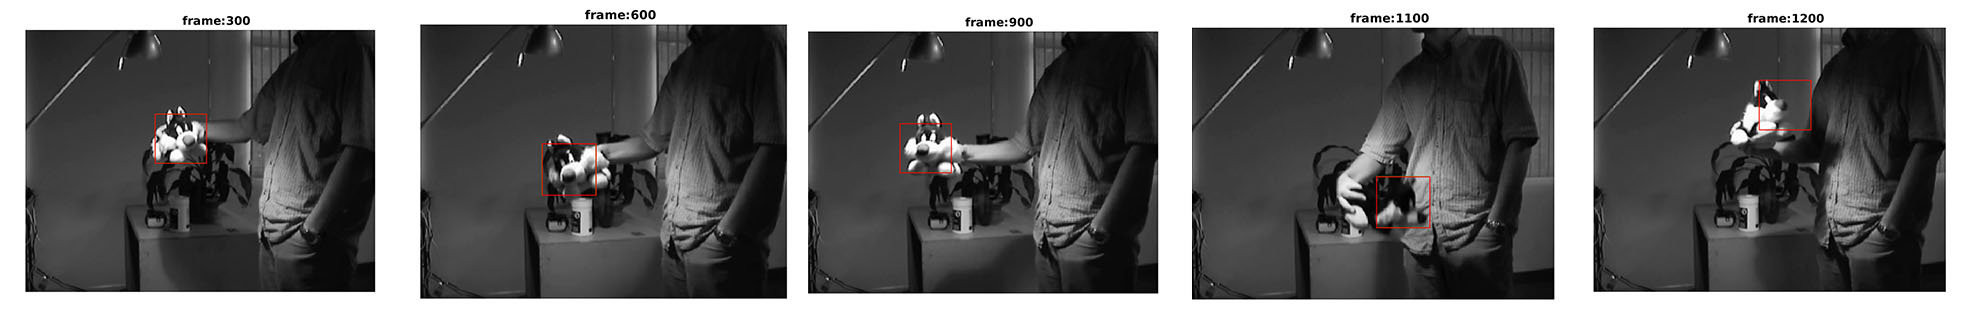
\includegraphics[width=6.5in]{./figures/p2-ext}
    \caption{The result of the tracking algorithm on the extended data set at frames 300,600,900,1100,1200. Note the slight green outline on frame 1100 and 1200}
\end{figure}
\subsection*{Q3.3}
Following is the images showcasing the result of \textbf{LucasKanadeAffine} at different frames. The red fills on the image are locations where we detect motions. 
\begin{figure}[H]
    \centering
    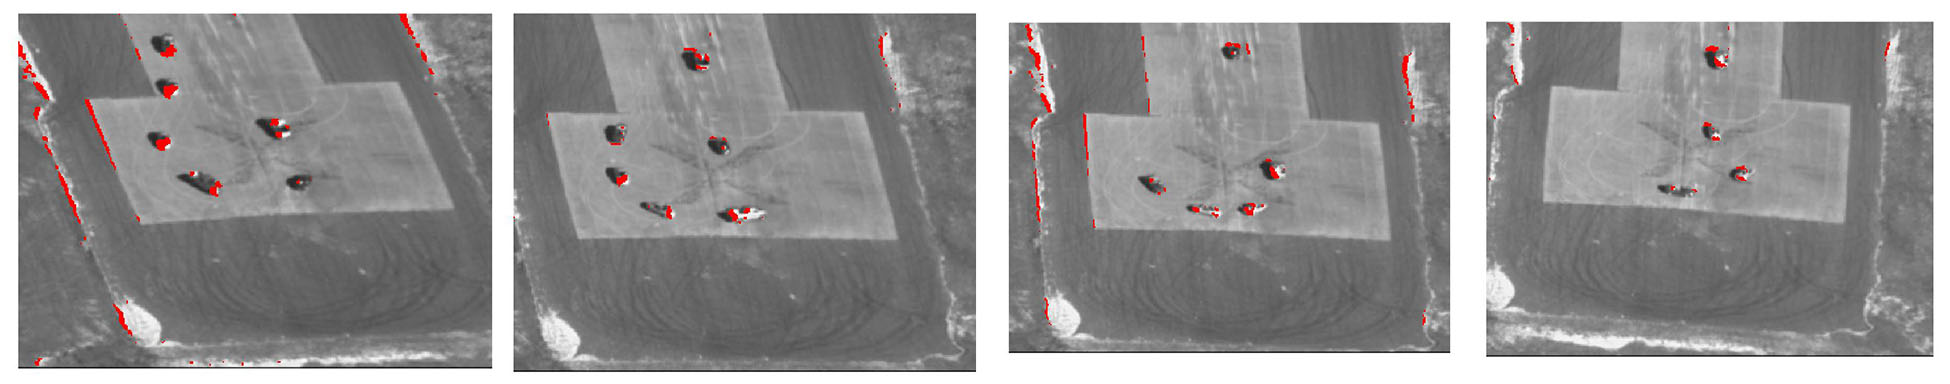
\includegraphics[width=6.5in]{./figures/p3}
    \caption{The result of the tracking algorithm at frames 30,60,90,120(left to right).}
\end{figure}
All the masks are saved in the file \textbf{aerialseqmasks.mat}
\end{document}